% THIS IS AN EXAMPLE DOCUMENT FOR VLDB 2012
% based on ACM SIGPROC-SP.TEX VERSION 2.7
% Modified by  Gerald Weber <gerald@cs.auckland.ac.nz>
% Removed the requirement to include *bbl file in here. (AhmetSacan, Sep2012)
% Fixed the equation on page 3 to prevent line overflow. (AhmetSacan, Sep2012)

\documentclass{vldb}
\usepackage[utf8]{inputenc} % Required for inputting international characters
\usepackage[T1]{fontenc} % Output font encoding for international characters
\usepackage{mathpazo} % Palatino font
\usepackage{graphicx}
\usepackage{subfig}
\usepackage{float}
\usepackage{listings}
\usepackage{amsmath,bm} 
\usepackage{balance}  % for  \balance command ON LAST PAGE  (only there!)

\tolerance=1
\emergencystretch=\maxdimen
\hyphenpenalty=10000
\hbadness=10000
\begin{document}

% ****************** TITLE ****************************************

\title{Effect of CapsuleNet Discriminator on GANs}%\titlenote{for use with vldb.cls}}

% possible, but not really needed or used for PVLDB:
%\subtitle{[Extended Abstract]
%\titlenote{A full version of this paper is available as\textit{Author's Guide to Preparing ACM SIG Proceedings Using \LaTeX$2_\epsilon$\ and BibTeX} at \texttt{www.acm.org/eaddress.htm}}}

% ****************** AUTHORS **************************************

% You need the command \numberofauthors to handle the 'placement
% and alignment' of the authors beneath the title.
%
% For aesthetic reasons, we recommend 'three authors at a time'
% i.e. three 'name/affiliation blocks' be placed beneath the title.
%
% NOTE: You are NOT restricted in how many 'rows' of
% "name/affiliations" may appear. We just ask that you restrict
% the number of 'columns' to three.
%
% Because of the available 'opening page real-estate'
% we ask you to refrain from putting more than six authors
% (two rows with three columns) beneath the article title.
% More than six makes the first-page appear very cluttered indeed.
%
% Use the \alignauthor commands to handle the names
% and affiliations for an 'aesthetic maximum' of six authors.
% Add names, affiliations, addresses for
% the seventh etc. author(s) as the argument for the
% \additionalauthors command.
% These 'additional authors' will be output/set for you
% without further effort on your part as the last section in
% the body of your article BEFORE References or any Appendices.

\numberofauthors{3} %  in this sample file, there are a *total*
% of EIGHT authors. SIX appear on the 'first-page' (for formatting
% reasons) and the remaining two appear in the \additionalauthors section.

\author{
% You can go ahead and credit any number of authors here,
% e.g. one 'row of three' or two rows (consisting of one row of three
% and a second row of one, two or three).
%
% The command \alignauthor (no curly braces needed) should
% precede each author name, affiliation/snail-mail address and
% e-mail address. Additionally, tag each line of
% affiliation/address with \affaddr, and tag the
% e-mail address with \email.
%
% 1st. author
\alignauthor
Raghava G. Dhanya\\
       \affaddr{Sir. M. Visvesvaraya Institute of Technology}\\
       \affaddr{Bangalore}\\
       \affaddr{Karnataka, India}\\
       \affaddr{raghava.dhanya@gmail.com}
% 2nd. author
\alignauthor Shashank S.\\
       \affaddr{Sir. M. Visvesvaraya Institute of Technology}\\
       \affaddr{Bangalore}\\
       \affaddr{Karnataka, India}\\
       \affaddr{mr.knhash@gmail.com}
% 3rd. author
\alignauthor
Abhijith C.\\
       \affaddr{Sir. M. Visvesvaraya Institute of Technology}\\
       \affaddr{Bangalore}\\
       \affaddr{Karnataka, India}\\
       \affaddr{abhijith4m0505@gmail.com}
}
% There's nothing stopping you putting the seventh, eighth, etc.
% author on the opening page (as the 'third row') but we ask,
% for aesthetic reasons that you place these 'additional authors'
% in the \additional authors block, viz.

% Just remember to make sure that the TOTAL number of authors
% is the number that will appear on the first page PLUS the
% number that will appear in the \additionalauthors section.


\maketitle

\begin{abstract}
Current advances in Generative Adversarial Networks allow us to generate near
realistic images but they are still quite distinguishable from actual photographs. The
technology is also not very amiable to changes in the orientation of images in
Convolutional Neural Networks(CNN). Additionally, the amount of data required to
train the network must be exhaustive, for example, in case different perspectives of a
face are required, the various perspectives must be explicitly present in the training
data to achieve the result. Thus the network requires humongous amounts of data.
In this project we propose a novel approach to accomplish the same task using
CapsNet. CapsNet employs a dynamic routing algorithm which replaces the
scalar-output feature detectors of the CNN with vector-output capsules. A capsule is
essentially a group of neurons describing a specific part of an object or image. Active
capsules at one level make predictions, via transformation matrices, for the
instantiation parameters of higher-level capsules. In essence, the CapsNet is the
reverse of the common Computer Graphics pipeline where we convert objects to their
renders. The CapsNet starts from the pixel level and works up towards the object.
We propose that the amount of data required to train a comparable model is very
small while it gives comparable, if not better, results.
\end{abstract}

\section{Introduction}
One of the main aspirations of Artificial Intelligence is to develop algorithms and techniques that enrich computers with ability to understand our world. Generative models are one of the most promising approaches towards achieving this goal.\par
A generative model is a mathematical or statistical model to generate all values of a phenomena. To train such a model, we first collect a large amount of data in some domain (e.g., think millions of images, sentences, or sounds, etc.) and then train a model to generate data like it.\par
A generative algorithm models how data was generated to classify a data instance. It poses the question: according to my generation hypotheses, which category is most likely to generate this data instance? A discriminative algorithm does not care about how the data was generated, it just classifies a given data instance; that is, given the features of a data instance, they predict a label or category to which that data belong. Discriminative models learn the boundary between classes while Generative models model the distribution of individual classes; that is, a generative model learns the joint probability distribution $p(x,y)$ while a discriminative model learns the conditional probability distribution $p(y|x)$, “probability of y given x”.\par
The trick is that the neural networks that we use as generating models have a significantly smaller number of parameters than the amount of data on which we train them, so the models are forced to effectively discover and internalize the essence of the data to generate it.\par
\noindent There are multiple approaches to build generative models 

\subsection{Generative adversarial networks}
One such model is the Generative adversarial networks (GANs), which are a class of generative algorithms used
in unsupervised machine learning, implemented by a system of two neural networks
competing in a zero-sum game framework. They were presented by Ian Goodfellow
et al. [12]. This technique can generate photographs that seem at least superficially
authentic to human observers, having many realistic features (though in tests people
can tell real from generated in some cases).

\label{sec:generative_adversarial_networks}
\begin{figure}[H]
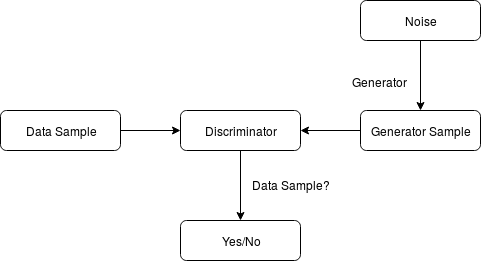
\includegraphics[width=\linewidth]{../Final_Report/images/vanillaGAN.png}
\caption{Vanilla Generative Adversarial Network}
\label{fig:gans}
\end{figure}

Generative Adversarial Networks, which we already discussed above, pose the training process as a game between two distinct networks: A neural network, called the generator, generates new instances of data, while the other, the discriminator, evaluates their authenticity; discriminator network tries to classify samples as either coming from the true distribution $p(x)$ or the model distribution $\hat{p}(x)$. Every time the discriminator notices a difference between the two distributions the generator adjusts its parameters slightly to make it go away, until at the end (in theory) the generator exactly reproduces the true data distribution and the discriminator is guessing at random, unable to find a difference.
The generator takes noise as input and attempts to produce an image that belongs to the real distribution; that is, it tries to fool the discriminator to accept it as real image. Discriminator takes a generated image or a real image as input and attempts to correctly classify the image as real or fake (generated).
To learn the distribution of the generator $p_g$ over data $\bm{x}$, we define a prior on input noise variables $p_{\bm{z}}(\bm{z})$, then represent a mapping to data space as $G(\bm{z}; \theta_g)$, where $G$ is a differentiable function represented by a neural network with parameters $\theta_g$. We define a second neural network $D(\bm{x}; \theta_d)$ that outputs a single scalar. $D(\bm{x})$ represents the probability that $\bm{x}$ came from the data rather than $p_g$. We train $D$ to maximize the probability of assigning the correct label to the training examples and samples of $G$. We simultaneously train $G$ to minimize $\log(1-D(G(\bm{z})))$.
This can be represented minimax game \\

\begin{multline} \label{eu_eqn}
\min_{G} \max_{D} V(D, G)=\mathbb{E}_{\bm{x} \sim p_{\text{data}}(\bm{x})}[\log D(\bm{x})]\\
+\mathbb{E}_{\bm{z} \sim p_{\bm{z}}(\bm{z})}[\log (1 - D(G(\bm{z})))]
\end{multline}


\subsection{Convolutional Neural Networks}
\begin{figure}[H]
\centering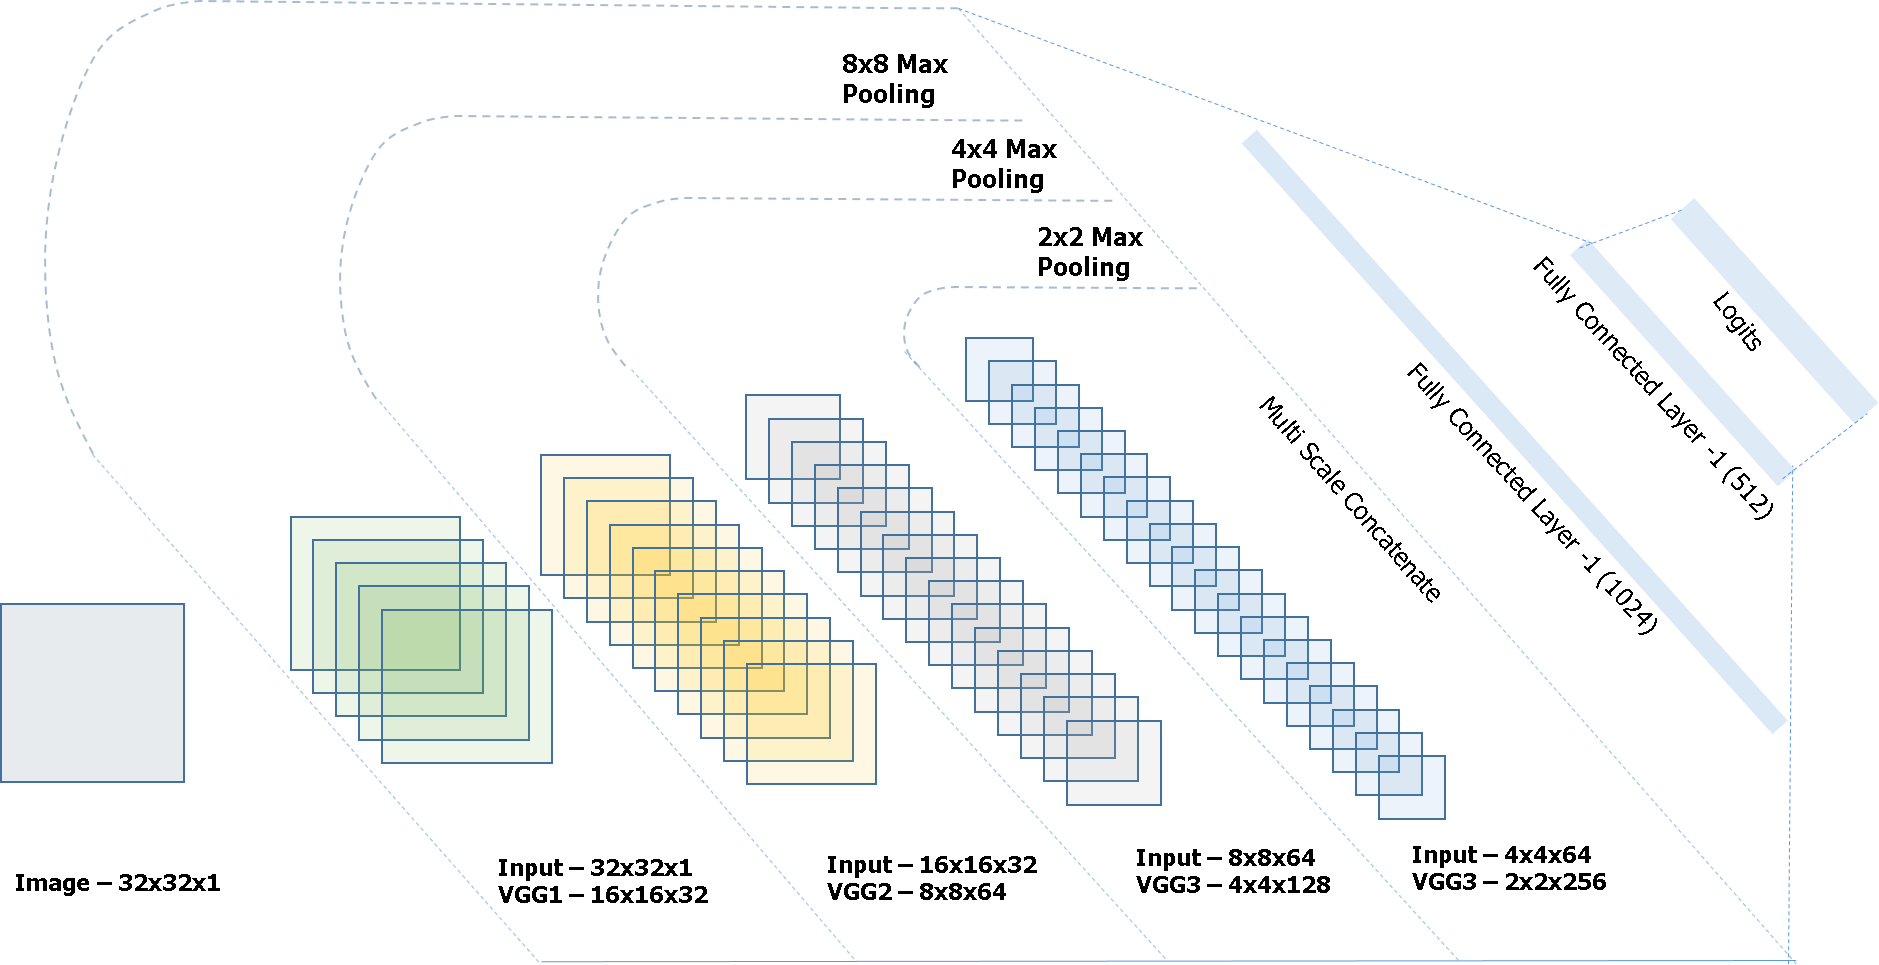
\includegraphics[width=\linewidth]{../Final_Report/images/CNN.png}
\caption{Convolutional Neural Network}
\label{fig:cnn}
\end{figure}
Before we can jump to understanding Capsule Networks, we need to know about Convolutional Neural Networks(CNNs). Convolutional neural networks are very similar to ordinary neural networks, they consist of neurons that have learn-able weights and biases. Each neuron receives inputs, performs a scalar product and possibly follows it with a nonlinearity. The entire network expresses a single differentiable score function: raw image pixels at one end to class scores at the other end. And they still have a loss function on the last layer.\par\bigskip
The major difference is that CNN explicitly assumes that the inputs are images, which allows us to encode certain properties in the architecture. These then make the forward functions more efficient to implement and significantly reduces the amount of parameters in the network.\par\bigskip
Ordinary neural networks don’t scale well to full images, for example, A colour image of dimensions of 150x150 (which is considered as low resolution by most people) has a shape (150,150,3), a fully connected neuron on first layer which receives this image would require 67500 weights. Unlike an ordinary neural network, the layers of a CNN have neurons arranged in 3 dimensions: width, height, depth as shown in figure \ref{fig:cnn}. The neurons in a layer will only be connected to a small region of the layer before it, instead of all of the neurons in a fully-connected manner. CNN  will reduce the full image into a single vector of class scores, arranged along the depth dimension.\par\bigskip
CNNs use a "Pooling" layer to reduce the spatial size of the input for each convolutional layer. The Pooling Layer operates independently on every depth slice of the input and resizes it spatially, generally using the MAX operation, hence pooling layer is sometimes referred to as Max Pooling layer.
% section convolutional_neural_network (end)

\subsection{Capsule Networks} % (fold)
\label{sec:capsule_networks}
“The pooling operation used in convolutional neural networks is a big mistake and the fact that it works so well is a disaster.” says Geoffrey Hinton, one of the founders of deep learning (Also known as Godfather of Deep Learning) and an inventor of numerous models and algorithms that are widely used today. CNNs perform exceptionally great when they are classifying images which are very close to the data set. If the images have rotation, tilt or any other different orientation then CNNs have poor performance. This problem is usually partially solved by adding different variations of the same image during training. But CNNs still require large amount of data to perform reasonably well. We use pooling after each layer to make it compute in reasonable time frames. But in essence, it also loses out the positional data.\par\bigskip
\begin{figure}[H]
\centering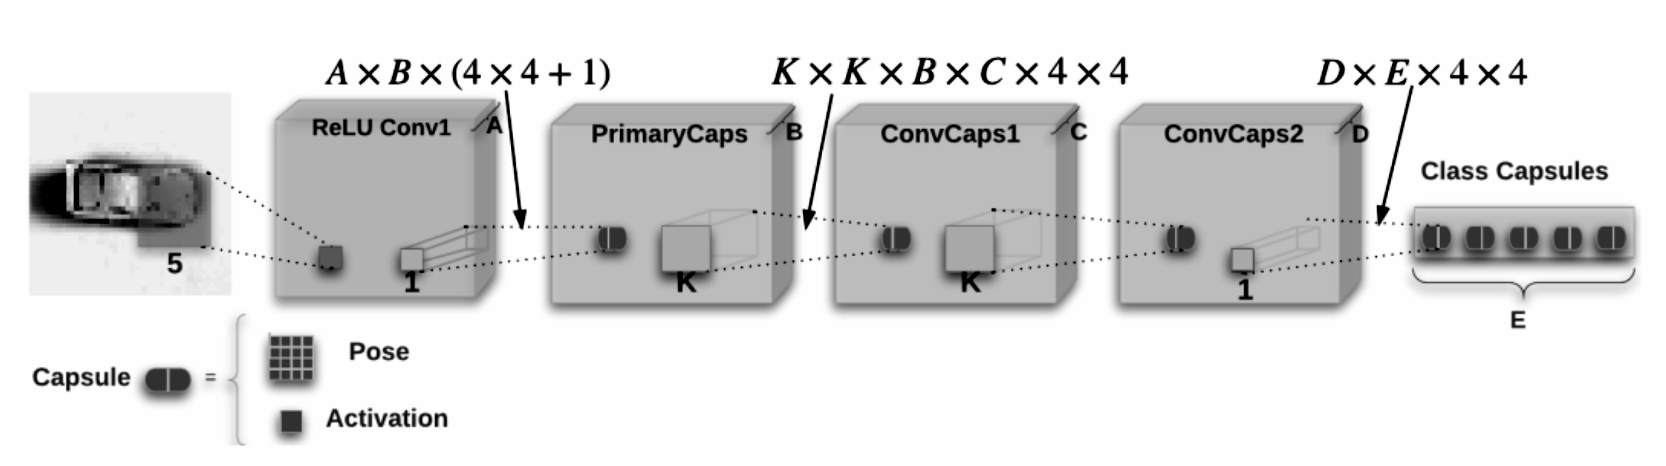
\includegraphics[width=\linewidth]{../Final_Report/images/caps.png}
\caption{Capsule Networks}
\label{fig:caps}
\end{figure}
What we need is not invariance but equivariance. Invariance makes a CNN tolerant to small changes in the viewpoint. Equivariance makes a CNN understand the rotation or proportion change and adapt itself accordingly so that the spatial positioning inside an image is not lost. This leads us to Capsule Networks.\par\bigskip
Capsule is a nested set of neural layers as shown in figure \ref{fig:caps}. Capsules are like cortical columns in human brains. Deep neural nets learn by back-propagation of errors over the entire network. In contrast real brains supposedly wire neurons by Hebbian principles: “units that fire together, wire together”. Capsules mimic Hebbian learning in the way that: “A lower-level capsule prefers to send its output to higher level capsules whose activity vectors have a big scalar product with the prediction coming from the lower-level capsule”. Capsules, combination of capsules encodes objects parts AND their relative positions, so an object instance can be accurately derived from the presence of the parts at the right locations, and not just their presence. Capsules produce equivariant features. Capsules predict the activity of higher-layer capsules to route information to right higher-layer capsules, this is called "Dynamic routing".


\section{Related work}
GANs were first introduced by Ian Goodfellow et al. [12] in Neural Information
Processing Systems 2014. The paper proposes a completely new framework for estimating
generative models via an adversarial process. In this process two models are
simultaneously trained. According to [12] the network has a generative model G that
captures the data distribution, and a discriminative model D that estimates the probability
that a sample came from the training data rather than G. This original work
by Ian Goodfellow uses fully connected neural networks in the generator and the discriminator.

\subsection{DCGAN}
Since GANs were introduced, there has been tremendous advancements in Deep Learning. A convolutional neural network (CNN, or ConvNet) \cite{imagenet} is a class of deep, feed-forward artificial neural networks that has successfully been applied to analyzing visual imagery. The convolution layer parameters consist of a set of learn-able filters, also called as kernels, which have a small receptive field, but they extend through the full depth of the input volume. As a result, the network learns filters that activate when it detects some specific type of feature at some spatial position in the input.
\par\bigskip
A breakthrough development that occurred in Adversarial Networks was the introduction of “Deep Convolutional Generative Adversarial Networks” by Alec Radford \textit{et al} \cite{dcgan}. DCGAN uses CNNs as generator and discriminator as shown in \ref{fig:dcgan}. He applied a list of empirically validated tricks as the substitution of pooling and fully connected layers with convolutional layers.
\par\bigskip
\begin{figure}[H]
\centering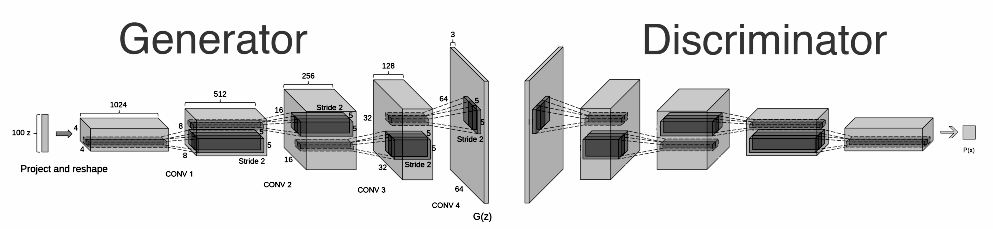
\includegraphics[width=\linewidth]{../Final_Report/images/dcgan.png}
\caption{Deep Convolutional Generative Adversarial Network}
\label{fig:dcgan}
\end{figure}
Today, most GANs are loosely based on the former shown DCGAN \cite{dcgan} architecture. Many papers have focused on improving the setup to enhance stability and performance. Many key insights was given by Salimans \textit{et al}. \cite{improvedgan}, like Usage of convolution with stride instead of pooling, Usage of Virtual Batch Normalization, Usage of Minibatch Discrimination in DD, Replacement of Stochastic Gradient Descent with Adam Optimizer [6], Usage of one-sided label smoothing.
\par\bigskip
% section dcgan (end)
\subsection{InfoGAN} % (fold)
\label{sec:infogan}
The power of the features encoded in the latent variables was further explored by Chen at al. \cite{infogan}. They propose an algorithm which is completely unsupervised, unlike previous approaches which involved supervision, and learns interpretable and disentangled representations on challenging datasets. Their approach only adds a negligible computation cost on top of GAN and is easy to train.
\par\bigskip

% section infogan (end)

\subsection{ACGAN} % (fold)
\label{sec:acgan}
Augustus Odena \textit{et al} \cite{acgan} came up a improved training of generative adversarial networks and variant of GAN with employing label conditioning that results in image samples exhibiting global coherence. ACGAN uses an auxiliary classifier to control the minimax game between generator and discriminator. In their work they demonstrate that adding more structure to the GAN latent space along with a specialized cost function results in higher quality samples
% section acgan (end)

\subsection{WGAN} % (fold)
\label{sec:wgan}
Another huge development came with the introduction of Wasserstein GANs by Martin Arjovsky \cite{wgan} . He introduced a new algorithm named WGAN, an alternative to traditional GAN training. In this new model, he showed that the stability of learning can be improved, remove problems like mode collapse, and provide good learning curves useful for debugging and hyperparameter searches.
\par\bigskip

This recently proposed Wasserstein GAN (WGAN) \cite{wgan} makes progress toward stable training of GANs, but sometimes can still generate only low-quality images or fail to converge. 
Ishaan Gulrajani with Martin Arjovsky proposed an alternative in \cite{improvedwgan} to fix the issues the previous GAN faced. This proposed method performs better than standard WGAN and enables stable training of a wide variety of GAN architectures with almost no hyperparameter tuning, including 101-layer ResNets \cite{deepresidual} and language models over discrete data.
\par\bigskip

% section wgan (end)
\subsection{Other GANs} % (fold)
\label{sec:other_gan}
Work by Mehdi Mirza \textit{et al}. \cite{congan} introduced the conditional version of GAN which can be constructed by simply feeding the data, y, we wish to condition on to both the generator and discriminator. The CGAN results were comparable with some other networks, but were outperformed by several other approaches – including non-conditional adversarial nets.
\par\bigskip

Sebastian Nowozin \textit{et al}. \cite{vardivmin} discussed the benefits of various choices of divergence functions on training complexity and the quality of the obtained generative models. They show that any f-divergence can be used for training generative neural samplers. 
\par\bigskip

Ming-Yu \textit{et al}. \cite{copgan} proposed coupled generative adversarial network (CoGAN) for learning a joint distribution of multi-domain images. The existing approaches requires tuples of corresponding images in different domains in the training data set. CoGAN can learn a joint distribution without any tuple of corresponding images.
\par\bigskip

% section other_gan (end)
\subsection{Capsule Neural Network} % (fold)
\label{sec:capsule_neural_network}
A big breakthrough in the field of Deep Learning came with the introduction of CapsNets or Capsule Networks \cite{capsnet} by the Godfather of Deep Learning, Geoffrey Hinton \textit{et al}. CNNs perform exceptionally great when they are classifying images which are very close to the data set. If the images have rotation, tilt or any other different orientation then CNNs have poor performance. A capsule is a group of neurons whose activity vector represents the instantiation parameters of a specific type of entity such as an object or an object part. They use the length of the activity vector to represent the probability that the entity exists and its orientation to represent the instantiation parameters. Active capsules at one level make predictions, via transformation matrices, for the instantiation parameters of higher-level capsules. When multiple predictions agree, a higher level capsule becomes active. They show that a discrimininatively trained, multi-layer capsule system achieves state-of-the-art performance on MNIST and is considerably better than a convolutional net at recognizing highly overlapping digits. To achieve these results they use an iterative routing-by-agreement mechanism: A lower-level capsule prefers to send its output to higher level capsules whose activity vectors have a big scalar product with the prediction coming from the lower-level capsule.

\section{Proposed Architecture}
The generator will use noise as input to generate faces. We will use random data as this noise. This ensures the data is unique and across the spectrum while retaining a normal distribution.
\par\bigskip

The CapsNet making up the discriminator consists of a small convolutional network to convert low level data in the form of pixels into an artifact called "pose". These poses can be anything, like nose, ear, eye, etc. These poses are then passed on as input to the later lower layers consisting of components called Capsules. A capsule is analogous to the human brain containing different modules to handle different tasks. The brain has a mechanism to route the information among the modules, to reach the best modules that can handle the information.
\par\bigskip

A capsule is a nested set of neural layers. Each capsule is able to handle one particular pose and communicate its calculation to other capsules which can use that calculation. This calculation is in the form of a probability prediction of the current pose that takes place in its logistic unit. This working is fundamentally different from convolutional networks, which utilizes Max Pooling. Max pooling selects the most active input node from the next layer to pass on the information. CapsNet on the other hand selects the next capsule based on which capsule would be capable of handling that information. This is called Dynamic routing. This results in invariance of information to the position and orientation of features in an object while ignoring the invariance in very low level features as, at the pixel level, this does not matter.
\par\bigskip


\begin{figure}[H]
\centering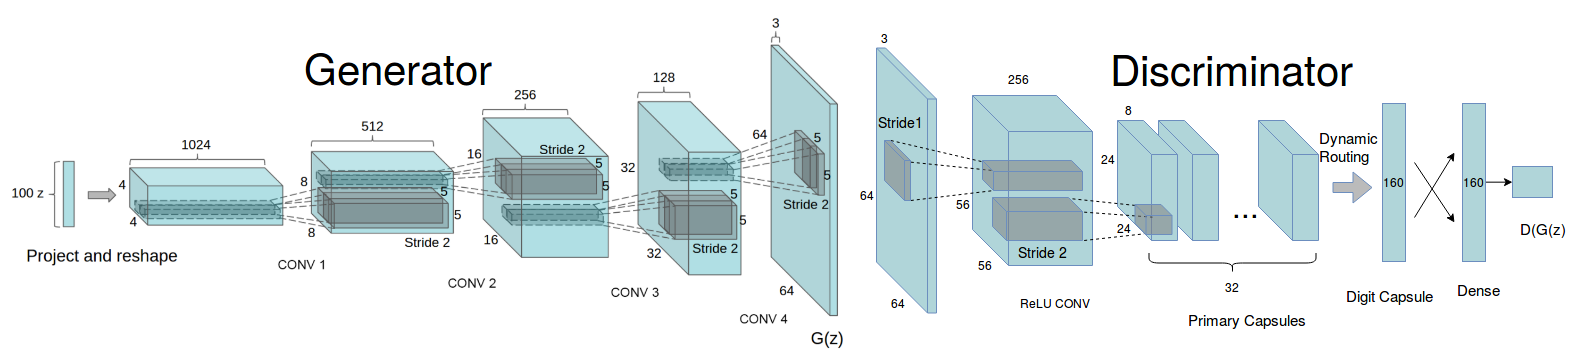
\includegraphics[width=\linewidth]{../Final_Report/images/CapsDCGAN.png}
\caption{Proposed architecture}
\label{fig:capsgan}
\end{figure}

\subsection{Generator} % (fold)
\label{sec:generator}
We use a deep convolutional generator model, which is similar to what DCGAN uses as generator. It starts with a latent vector or noise of shape 100 which connects to a densely connected neural layer. We then use Reshape layer which reshapes it to an (8, 8, 128) matrix and which is then sent to the batch normalization layer. We later perform up-sampling by using DeConv (De-Convolutional layer: transposed convolutional layer) layer. DeConv layer is internally implemented by an up-sampling layer and a convolutional layer. We perform DeConv two more times to get the shape of the image as expected, which should be (64, 64, 3), which stands for a 64x64 RGB image.
\begin{figure}[H]
\centering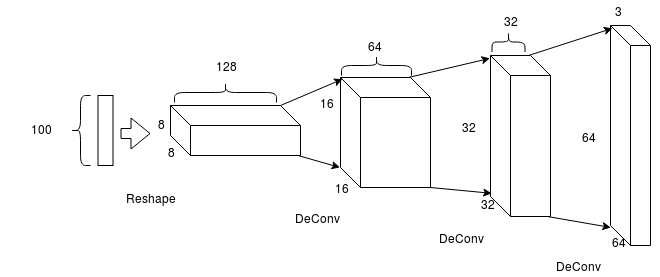
\includegraphics[width=\linewidth]{../Final_Report/images/Generator.png}
\caption{Generator architecture}
\label{fig:generator}
\end{figure} 

% section generator (end)


\subsection{Discriminator} % (fold)
\label{sec:discriminator}
The discriminator in the original models is replaced by our modification of CapsNet. We use a binary classifier CapsNet to distinguish between real and fake images. 

\par\bigskip
The CapsNet has 2 parts: encoder and decoder. The first 3 layers are encoder, and the second 3 are decoder:

Layer 1. Convolutional layer
Layer 2. PrimaryCaps layer
Layer 3. DigitCaps layer
Layer 4. Fully connected \#1
Layer 5. Fully connected \#2
Layer 6. Fully connected \#3

In our implementation, we do not use the decoder layers as we do not need the reconstruction aspects of the network for classification. Hence only the encoder layers are used.
\par\bigskip
The encoding part of the network takes as input a digital image of 64x64 and learns to encode it into a vector of 16 dimensions of instantiation parameters, this is where the capsules do their job. The output of the network during prediction is a 10-dimensional vector of the lengths of the DigitCaps' outputs.

% Discriminator image

\subsubsection{Layer 1: Convolutional Layer} % (fold)
\label{sub:layer_1_convolutional_layer}
\noindent Input: 64x64 image (three color channel).
\\Output: 56x56x256 tensor.
\\Number of parameters: 62464.

\par\bigskip The work of the convolutional layer consists of detecting the basic functions in the 2D image. In the CapsNet system, the convolutional layer has 256 kernels of size 9x9x1 and stride of 1, followed by the activation function, ReLU. To calculate the number of parameters, we must also remember that each kernel in a convolutional layer has 1 bias term. Therefore, this layer has (9 x 9 x 3 x 256 + 256 =) 62464 trainable parameters in total.

% subsection layer_1_convolutional_layer (end)

\subsubsection{Layer 2: PrimaryCaps Layer} % (fold)
\label{sub:layer_2_primarycaps_layer}
\noindent Input: 56x56x256 tensor.
\\Output: 24x24x8x32 tensor.
\\Number of parameters: 5308672.

\par This layer has 32 primary capsules whose job is to take basic features detected by the convolutional layer and produce combinations of the features. The layer has 32 “primary capsules” that are very similar to convolutional layer in their nature. Each capsule applies eight 9x9x256 convolutional kernels to the 56x56x256 input volume and therefore produces 24x24x8 output tensor. Since there are 32 such capsules, the output volume has shape of 24x24x8x32. Doing calculation similar to the one in the previous layer, we get (9 x 9 x 256 x 256 + 256 =) 5308672 trainable parameters in this layer.

% subsection layer_2_primarycaps_layer (end)

\subsubsection{Layer 3: DigitCaps Layer} % (fold)
\label{sub:layer_3_digitcaps_layer}
\noindent Input: 24x24x8x32 tensor.
\\Flattened to: 147456
\\Output: 1x1 matrix.
\\Number of parameters: 1497600.

\par We have a 3 hidden-layer densely connected neural network which takes the flattened input to give a binary classification output of 1x1. Each hidden layer consists of 160 neurons. From the flattened input we get the input of size 147456 which is connected densely to the first hidden layer. Thus the weights in the first layer turn out to be (147456 x 160 + 160 =)  23593120 in number. The first hidden layer is connected to the second hidden layer densely, similarly the second and the third. Therefore there are (160 x 160 + 160 =) 25760 trainable parameters for the second and third hidden layers. 
\par The last last hidden layer is connected to a output layer with one neuron, which essentially gives the binary classification result. Its parameters are (160 x 1 + 1 =) 161 in number. 

\section{Implementations}
The first step is to implement the state-of-the-art in image regeneration to guage the improvements. We use DCGAN to start of with. The results of the training and testing will be recorded to compare it with the results of our CapsNet-based approach later. We will be using CapsNet as the underlying technology to implement our GAN (CapsGAN). The goal is to replace the CNN inside DCGAN with CapsNet and compare the results. The GAN internally consists of two components - a generator and a discriminator - which we build out of CapsNet. The discriminator is initially trained separately to distinguish real and fake data, and later they work together to improve upon their performance by acting as adversaries.
\par


During the course of our research we were forced to conclude that building a CapsNet based generator was not feasible. A fundamental aspect of a GAN is back-propagation in the discriminator which is not possible to replicate in the generator. Hence we implemented just the discriminator in CapsNet. 
\par

We concentrated on four networks: DCGAN, WGAN, ACGAN and InfoGAN. Our training laboratory was Colloboratory - the cloud machine learning research platform. We trained each network individually for 20,000 epochs each. \\
For our preliminary training we used the MNIST dataset. The MNIST dataset is a large dataset of handwritten digits commonly used for image processing training tasks. Each of the networks had it's discriminator augmented with the CapsNet code. The networks with the CapsNet discriminator were then individually trained on the same dataset, for 20,000 epochs each. Overall, it took us a few days to train all the networks and gather all the data.


\subsection{Network Architectures} % (fold)
\label{sec:network_architectures}

\subsubsection{Generator} % (fold)
\label{sub:Generator}
\begin{figure}[H]
\centering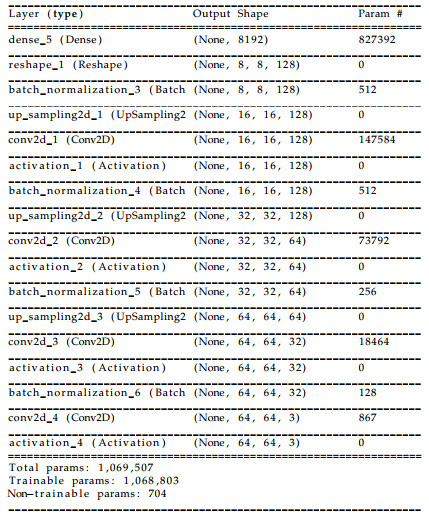
\includegraphics[width=\linewidth]{../Final_Report/images/generator_layers.png}
\caption{Generator layers}
\label{fig:generator}
\end{figure} 
\newpage
\subsubsection{Discriminator} % (fold)
\label{sub:Discriminator}
\begin{figure}[H]
\centering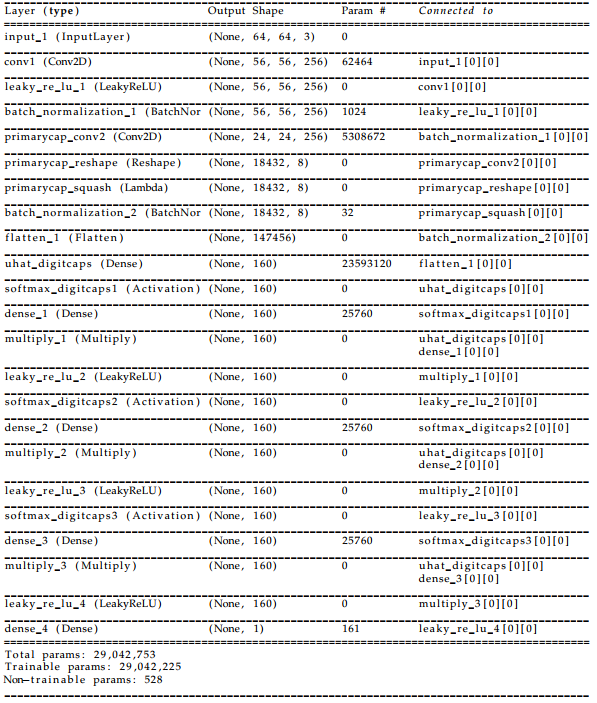
\includegraphics[width=\linewidth]{../Final_Report/images/discriminator_layers.png}
\caption{Discriminator layers}
\label{fig:discriminator_layers}
\end{figure} 

\section{Results}
\subsection{Training} % (fold)
\label{sec:training}

% section training (end)
Our research consisted of four networks: ACGAN, DCGAN, InfoGAN and WGAN. Each of the networks was trained for 20,000 epochs each. The training period for the individual networks took anywhere between a few hours and a couple of days. For each network, we logged a few key metrics, mainly the Generator Loss (GLoss), Discriminator Loss (DLoss) and the Accuracy (Acc). 
\par\bigskip
Below we show graphically the performance of the (four) classical networks as compared to the CapsNet discriminator augmented networks.

\begin{figure}[H]
    \centering
    \subfloat[Classical ACGAN]{{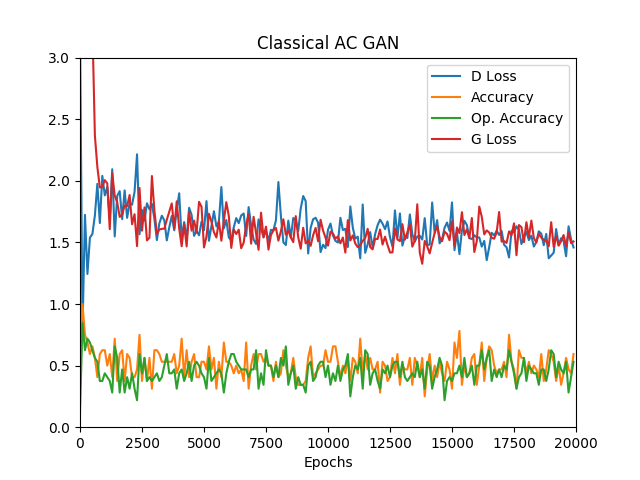
\includegraphics[width=.45\linewidth]{../Final_Report/images/plots/classacgan.png} }}%
    \qquad
    \subfloat[CapsNet ACGAN]{{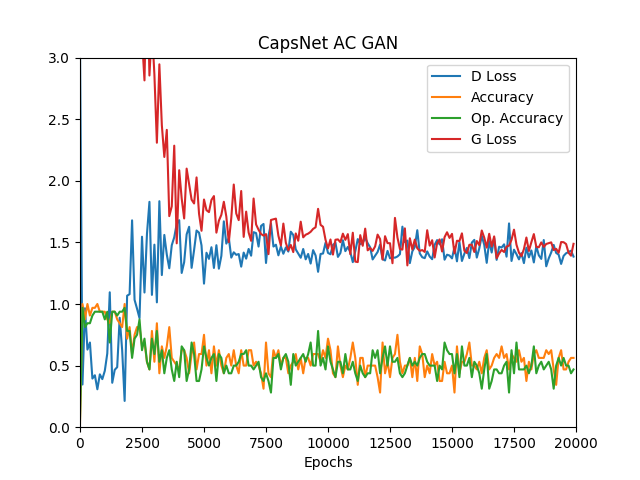
\includegraphics[width=.45\linewidth]{../Final_Report/images/plots/capsacgan.png} }}%
    \caption{ACGAN metrics}%
    \label{fig:acgan_metric}%
\end{figure}

\begin{figure}[H]
    \centering
    \subfloat[Classical DCGAN]{{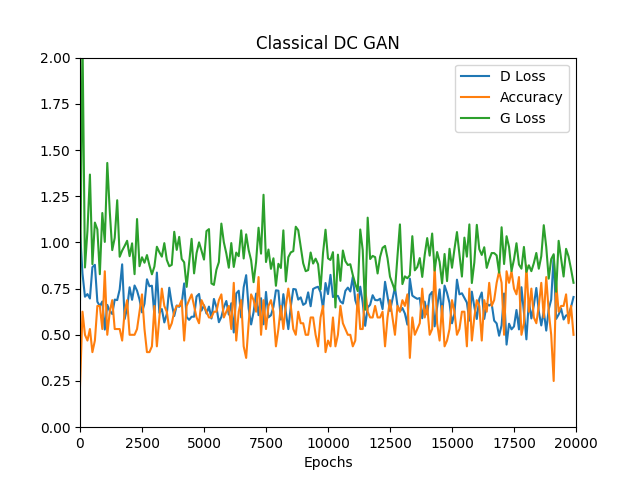
\includegraphics[width=.45\linewidth]{../Final_Report/images/plots/classdcgan.png} }}%
    \qquad
    \subfloat[CapsNet DCGAN]{{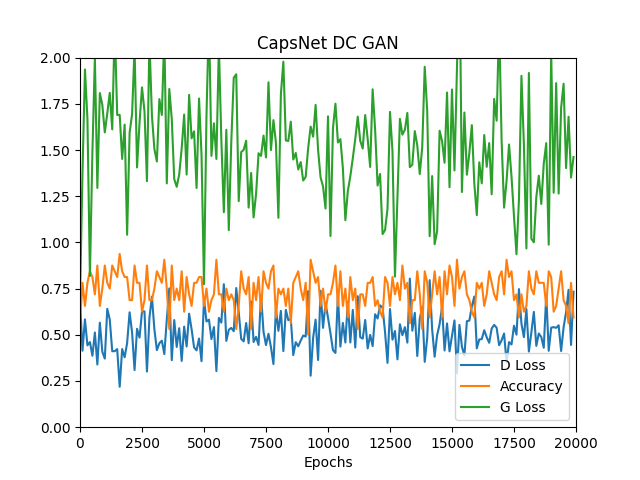
\includegraphics[width=.45\linewidth]{../Final_Report/images/plots/capsdcgan.png} }}%
    \caption{DCGAN metrics}%
    \label{fig:dcgan_metric}%
\end{figure}

\begin{figure}[H]
    \centering
    \subfloat[Classical InfoGAN]{{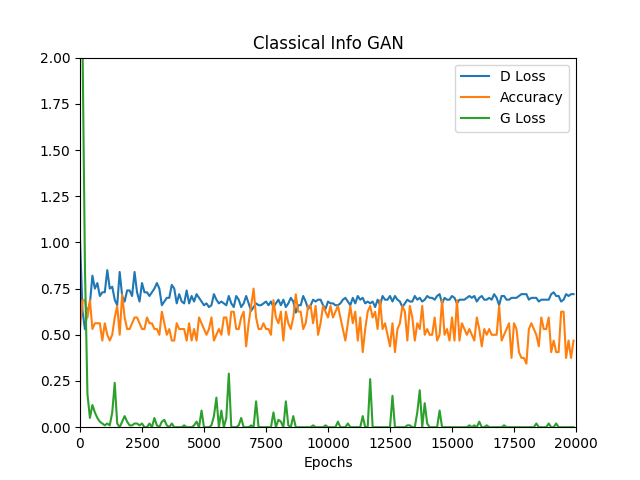
\includegraphics[width=.45\linewidth]{../Final_Report/images/plots/classinfogan.png} }}%
    \qquad
    \subfloat[CapsNet InfoGAN]{{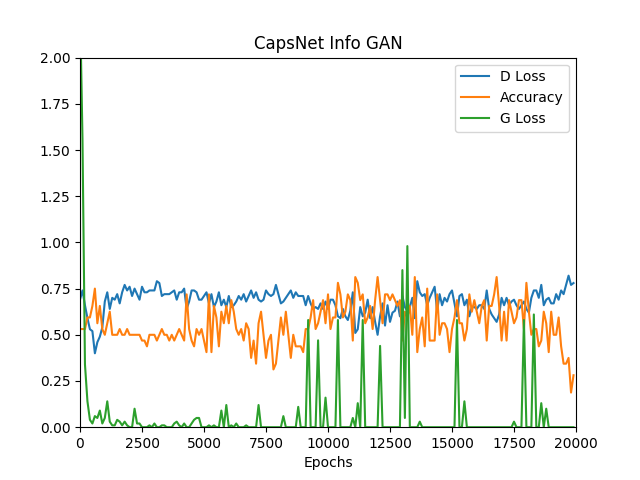
\includegraphics[width=.45\linewidth]{../Final_Report/images/plots/capsinfogan.png} }}%
    \caption{InfoGAN metrics}%
    \label{fig:infogan_metric}%
\end{figure}

\begin{figure}[H]
    \centering
    \subfloat[Classical WGAN]{{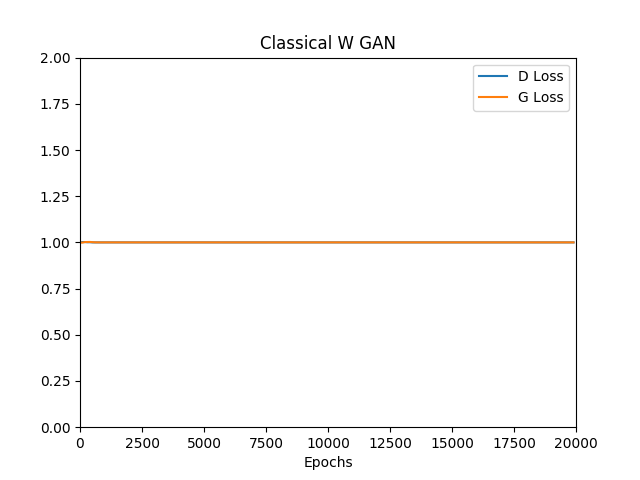
\includegraphics[width=.45\linewidth]{../Final_Report/images/plots/classwgan.png} }}%
    \qquad
    \subfloat[CapsNet WGAN]{{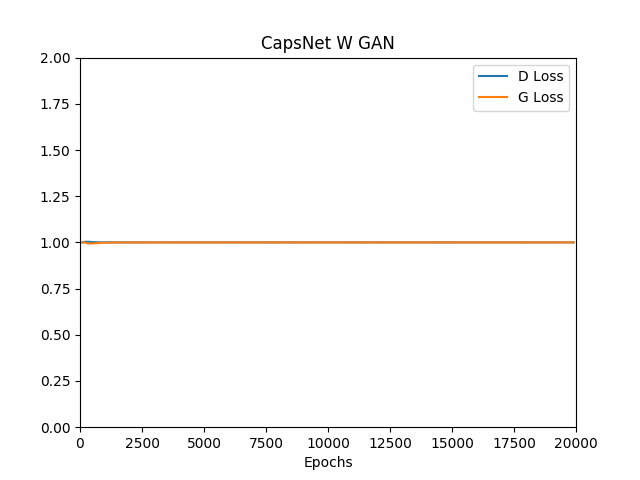
\includegraphics[width=.45\linewidth]{../Final_Report/images/plots/capswgan.png} }}%
    \caption{WGAN metrics}%
    \label{fig:wgan_metric}%
\end{figure}

The metrics of WGAN are at a smaller scale, so below is a comparison at the lower scale.

\begin{figure}[H]
    \centering
    \subfloat[Classical WGAN]{{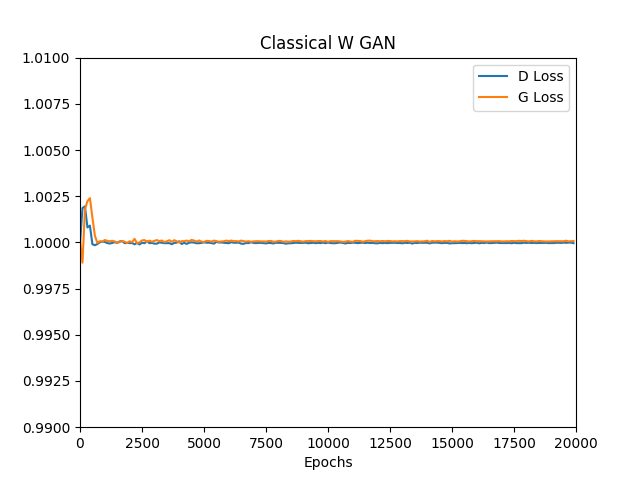
\includegraphics[width=.45\linewidth]{../Final_Report/images/plots/classwgan-zoomed.png} }}%
    \qquad
    \subfloat[CapsNet WGAN]{{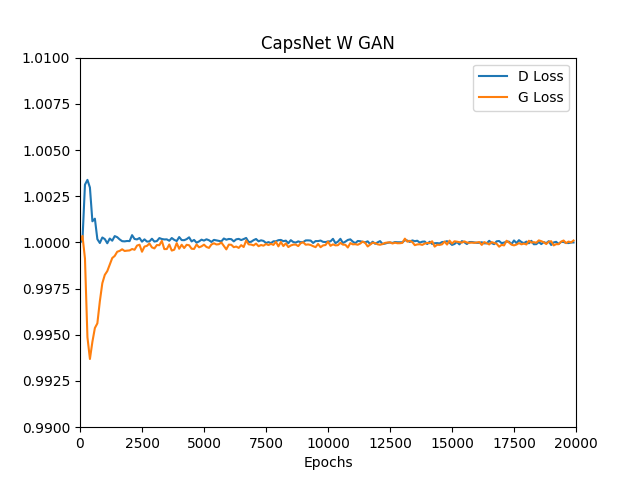
\includegraphics[width=.45\linewidth]{../Final_Report/images/plots/capswgan-zoomed.png} }}%
    \caption{WGAN metrics - zoomed}%
    \label{fig:wgan_metric_zoomed}%
\end{figure}
\par\bigskip

A preliminarily analysis of the data shows us that our CapsNet augmented networks, hence-forth referred to as the network name prefixed with "Caps", perform comparably with the classical architectures. 
\par\bigskip

Under ACGAN we see that CapsACGAN starts off with very high variance in GLoss and DLoss. Over the course of 20,000 epochs, the variance gradually reduces to match the Classical ACGAN metrics at the end. Accuracy of CapsACGAN, on the other hand, quickly stabilizes to meet classical ACGAN metrics. As a side note, ACGAN was the fastest trained network, taking roughly three hours to complete 20,000 epochs.
\par\bigskip

DCGAN and InfoGAN are interesting in the sense that they show a remarkable shift in the GLoss metric. Even though it seems as if augmenting DCGAN with CapsNet discriminator leads to increase in GLoss, a closer look reveals that increased variation leads to faster learning of the generator network. Accuracy and DLoss follow their classical counterpart closely.
\par\bigskip

WGAN happens to be the best and state-of-the-art. Consequently, the variance in the metrics were at a much smaller scale, that is, the network is designed to be more stabilized and balanced but this also leads to slower learning, we can see that adding CapsNet discriminator speeds this up by adding slightly more variance while the network is still balanced. We had to zoom-in to notice the difference between the metrics. We see that an initial burst of high variance quickly stabilizes to trace a path closely matching the classical architecture.
\par\bigskip


\subsection{Generation} % (fold)
\label{sec:generation}
At the end of every epoch we saved the outputs of the generator. Here we show the outputs of generator of four networks after 20,000 epochs for comparison.
\begin{figure}[H]
    \centering
    \subfloat[Classical ACGAN]{{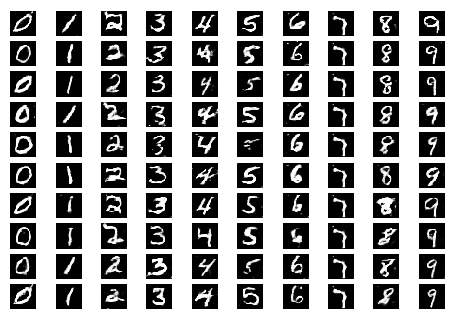
\includegraphics[width=.45\linewidth]{../Final_Report/images/generation_outputs/acgan.png} }}%
    \qquad
    \subfloat[CapsNet ACGAN]{{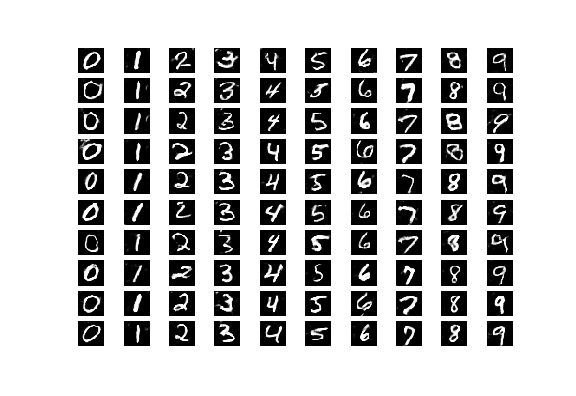
\includegraphics[width=.45\linewidth]{../Final_Report/images/generation_outputs/acgan_caps.png} }}%
    \caption{ACGAN outputs}%
    \label{fig:acgan_gen}%
\end{figure}
As expected from the metrics the ACGAN and CapsACGAN produce very similar outputs.
\begin{figure}[H]
    \centering
    \subfloat[Classical DCGAN]{{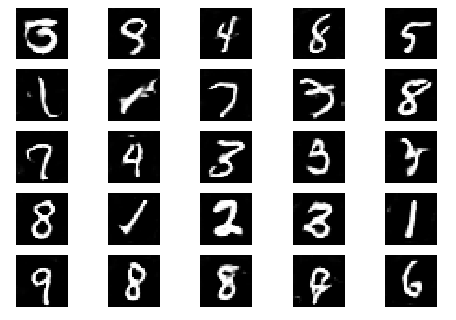
\includegraphics[width=.45\linewidth]{../Final_Report/images/generation_outputs/dcgan.png} }}%
    \qquad
    \subfloat[CapsNet DCGAN]{{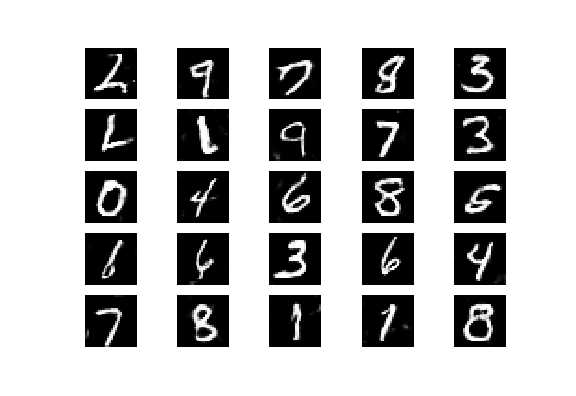
\includegraphics[width=.45\linewidth]{../Final_Report/images/generation_outputs/dcgan_caps.png} }}%
    \caption{DCGAN outputs}%
    \label{fig:dcgan_gen}%
\end{figure}
The outputs of DCGAN and CapsDCGAN are almost indistinguishable but a closer look reveals that CapsDCGAN produces more clear outputs and more percentage of CapsDCGAN outputs look real.

\begin{figure}[H]
    \centering
    \subfloat[Classical InfoGAN]{{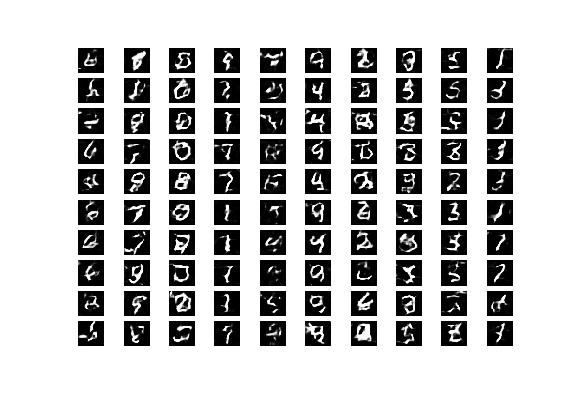
\includegraphics[width=.45\linewidth]{../Final_Report/images/generation_outputs/infogan.png} }}%
    \qquad
    \subfloat[CapsNet InfoGAN]{{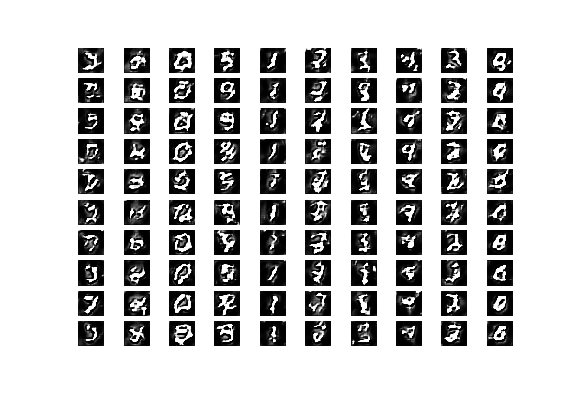
\includegraphics[width=.45\linewidth]{../Final_Report/images/generation_outputs/infogan_caps.png} }}%
    \caption{InfoGAN outputs}%
    \label{fig:infogan_gen}%
\end{figure}
Even though the CapsInfoGAN output looks structurally better and has learned faster but it is more noisier than that of the InfoGAN.
\begin{figure}[H]
    \centering
    \subfloat[Classical WGAN]{{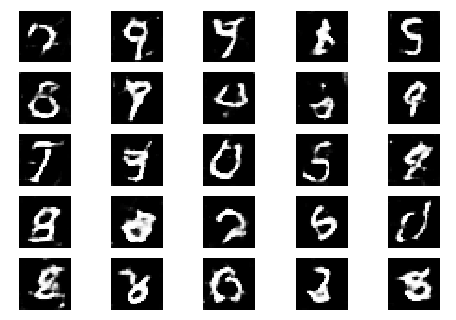
\includegraphics[width=.45\linewidth]{../Final_Report/images/generation_outputs/wgan.png} }}%
    \qquad
    \subfloat[CapsNet WGAN]{{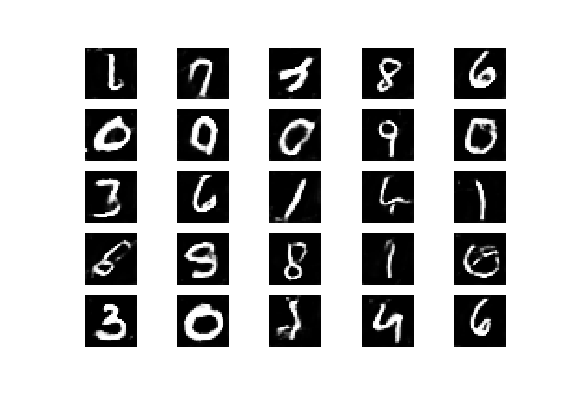
\includegraphics[width=.45\linewidth]{../Final_Report/images/generation_outputs/wgan_caps.png} }}%
    \caption{WGAN outputs}%
    \label{fig:wgan_gen}%
\end{figure}
Finally in the WGAN outputs we can clearly see that CapsWGAN produces clear and better outputs, hence has learned more quickly than the WGAN. 

\section{Conclusions}
During the course of this project, we wished to replicate the results of the existing state-of-the-art in Generative Models. We implemented a few different versions of GANs with CapsNet. Our motivating assumption was that CapsNet would provide a performance improvement. We based this on the idea that it is more capable of understanding the variances in objects. This in turn should lead to lower data requirements during training of the model and consequently lower power consumption. 
\par\bigskip 

We provide a comparison between our novel CapsNet-based approach and other implementations of GAN for the same task. To observe this we augment the code of a few GANs, namely ACGAN, InfoGAN, DCGAN and WGAN, by implementing the discriminator with CapsNet. We decided to work with a few standard metrics such as Discriminator Loss, Generator Loss and Accuracy to measure its training performance. The data while training was captured and visualized in the form of graphs.
\par\bigskip 

% Conclusion from results and analysis


In conclusion, we can confidently state that augmenting the GANs with CapsNet was a fruitful endeavor. The CapsNet helped to reduce th training overhead considerably when compared to classical networks while providing remarkably similar results. Our research shows that embedding CapsNet into the GAN does not degrade its performance and, in certain cases, improves upon it.
%\end{document}  % This is where a 'short' article might terminate

% ensure same length columns on last page (might need two sub-sequent latex runs)
\balance

%ACKNOWLEDGMENTS are optional
\section{Acknowledgments}
\noindent Every project requires some form of help. In this section , we would like to thank the people who helped us make this project a reality.
\par\bigskip
We would like to thank \textbf{Prof. Dilip K. Sen}, Head of the department, CSE, for his support. Our heartfelt gratitude to our guide, \textbf{Mrs. Sushila Shidnal}, for her invaluable guidance, encouragement and advice. We take this opportunity to thank all the teaching as well as non-teaching staff for their support and motivation. 
\par\bigskip
We thank \textbf{Google} for \textbf{Google Colaboratory}, where we ran most of our Deep Learning model training.
\par\bigskip
% The following two commands are all you need in the
% initial runs of your .tex file to
% produce the bibliography for the citations in your paper.
\bibliographystyle{abbrv}
\bibliography{vldb}  % vldb_sample.bib is the name of the Bibliography in this case
% You must have a proper ".bib" file
%  and remember to run:
% latex bibtex latex latex
% to resolve all references
%APPENDIX is optional.
% ****************** APPENDIX **************************************
% Example of an appendix; typically would start on a new page
%pagebreak



\end{document}
